Quark versus gluon tagging is sensitive to the detailed modeling of perturbative and non-perturbative effects involved with fragmentation.  
We compare images and image classification performance with two very different fragmentation models.  
Figure~\ref{fig:avg:pythiasherpa} shows the average image (differences) between quark and gluon jets simulated with 
\textsc{Pythia} 8 and with \textsc{Herwig++}.  
The radiation pattern inside gluon jets is similar between the two models, whereas there are larger differences for quark jets.  
In particular, quark and gluon jets are more different according to \textsc{Pythia} 8 relative to \textsc{Herwig++}.  
This is observed with the CNN in Fig.~\ref{fig:pythiasherpa}.  
As gluon jets in \textsc{Herwig++} are more similar to quark jets than in \textsc{Pythia} 8, 
any observable (including the CNN tagger output) tends to have less discrimination power when tested in \textsc{Herwig++}.
The training sample determines the nature of the observable the CNN tagger learns. 
By comparing the CNN tagger trained on \textsc{Pythia} 8 events with the one trained on \textsc{Herwig++} events
using the same test sample (\textsc{Pythia} 8),
we see a smaller discrepancy, indicating that the learned feature is not strongly sensitive 
to the difference between \textsc{Pythia} 8 and \textsc{Herwig++}.
\textsc{Pythia} 8 and \textsc{Sherpa} produce relatively similar images and so unsurprisingly, 
the CNN performance is similar when trained/tested on either of these generators.  
As also noted by Ref.~\cite{Barnard:2016qma}, when generators produce different images, 
the CNN returns a different performance when training and testing with images from various simulators.  
However, if the same network is used for testing and only the training sample is varied, 
the gap in performance is mostly removed (see also~\cite{Komiske:2016rsd}).  
One explanation is that the network is learning robust features for quark versus gluon tagging, 
but the degree to which the features are expressed in the radiation patterns varies between generators.

%As alternative to the baseline \textsc{Pythia} 8 sample described in Section~\ref{sec:images},  we consider a dijet sample generated with \textsc{SHERPA} (v2.2.0)~\cite{Gleisberg:2008ta} and the CT10 PDF set. Interestingly, the models themselves result in similar images, shown in Figure~\ref{fig:avg:truthtrack}, and not surprisingly, Figure~\ref{fig:pythiasherpa} shows that the tagger performance is also similar.

\begin{figure}[tbp]
\begin{center}
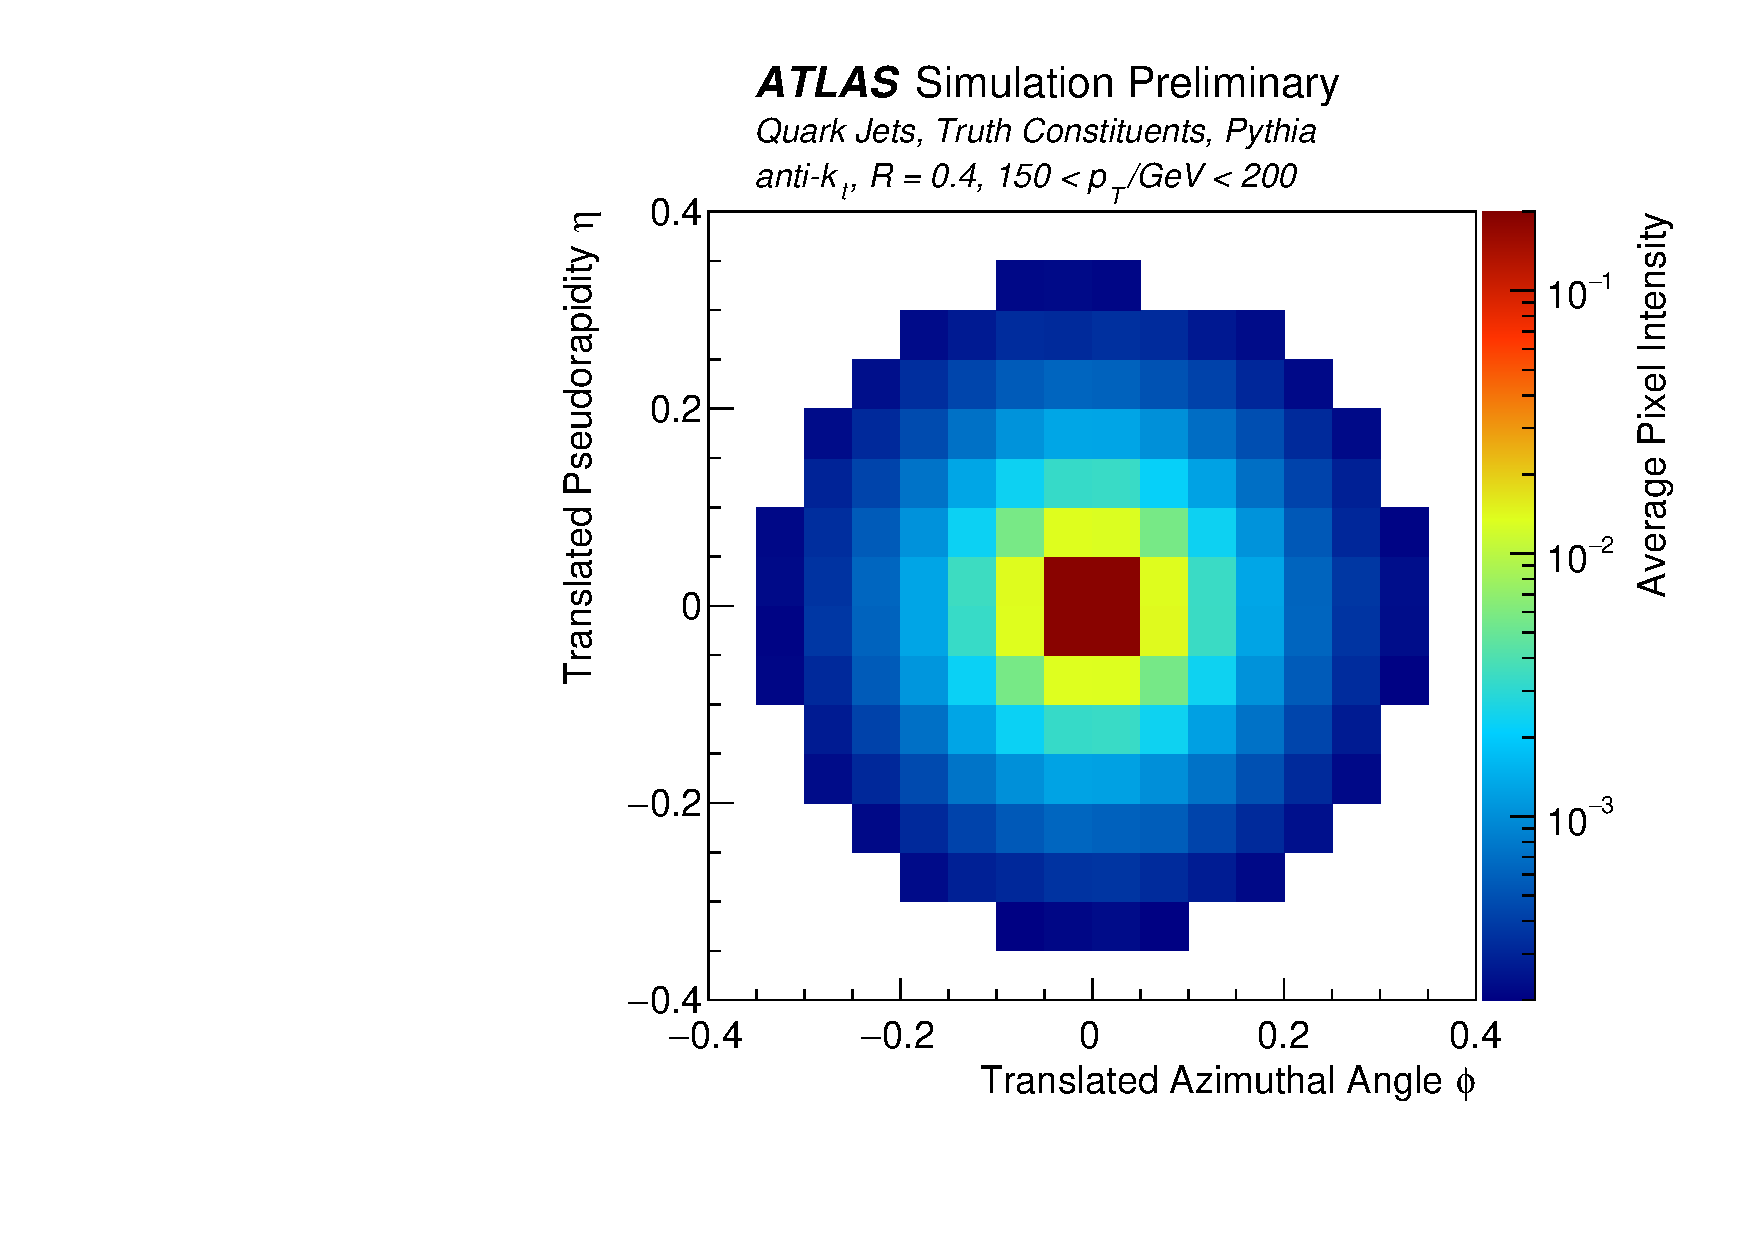
\includegraphics[width=0.33\textwidth]{figures/pythiasherpa/quark_truth_pythia.pdf}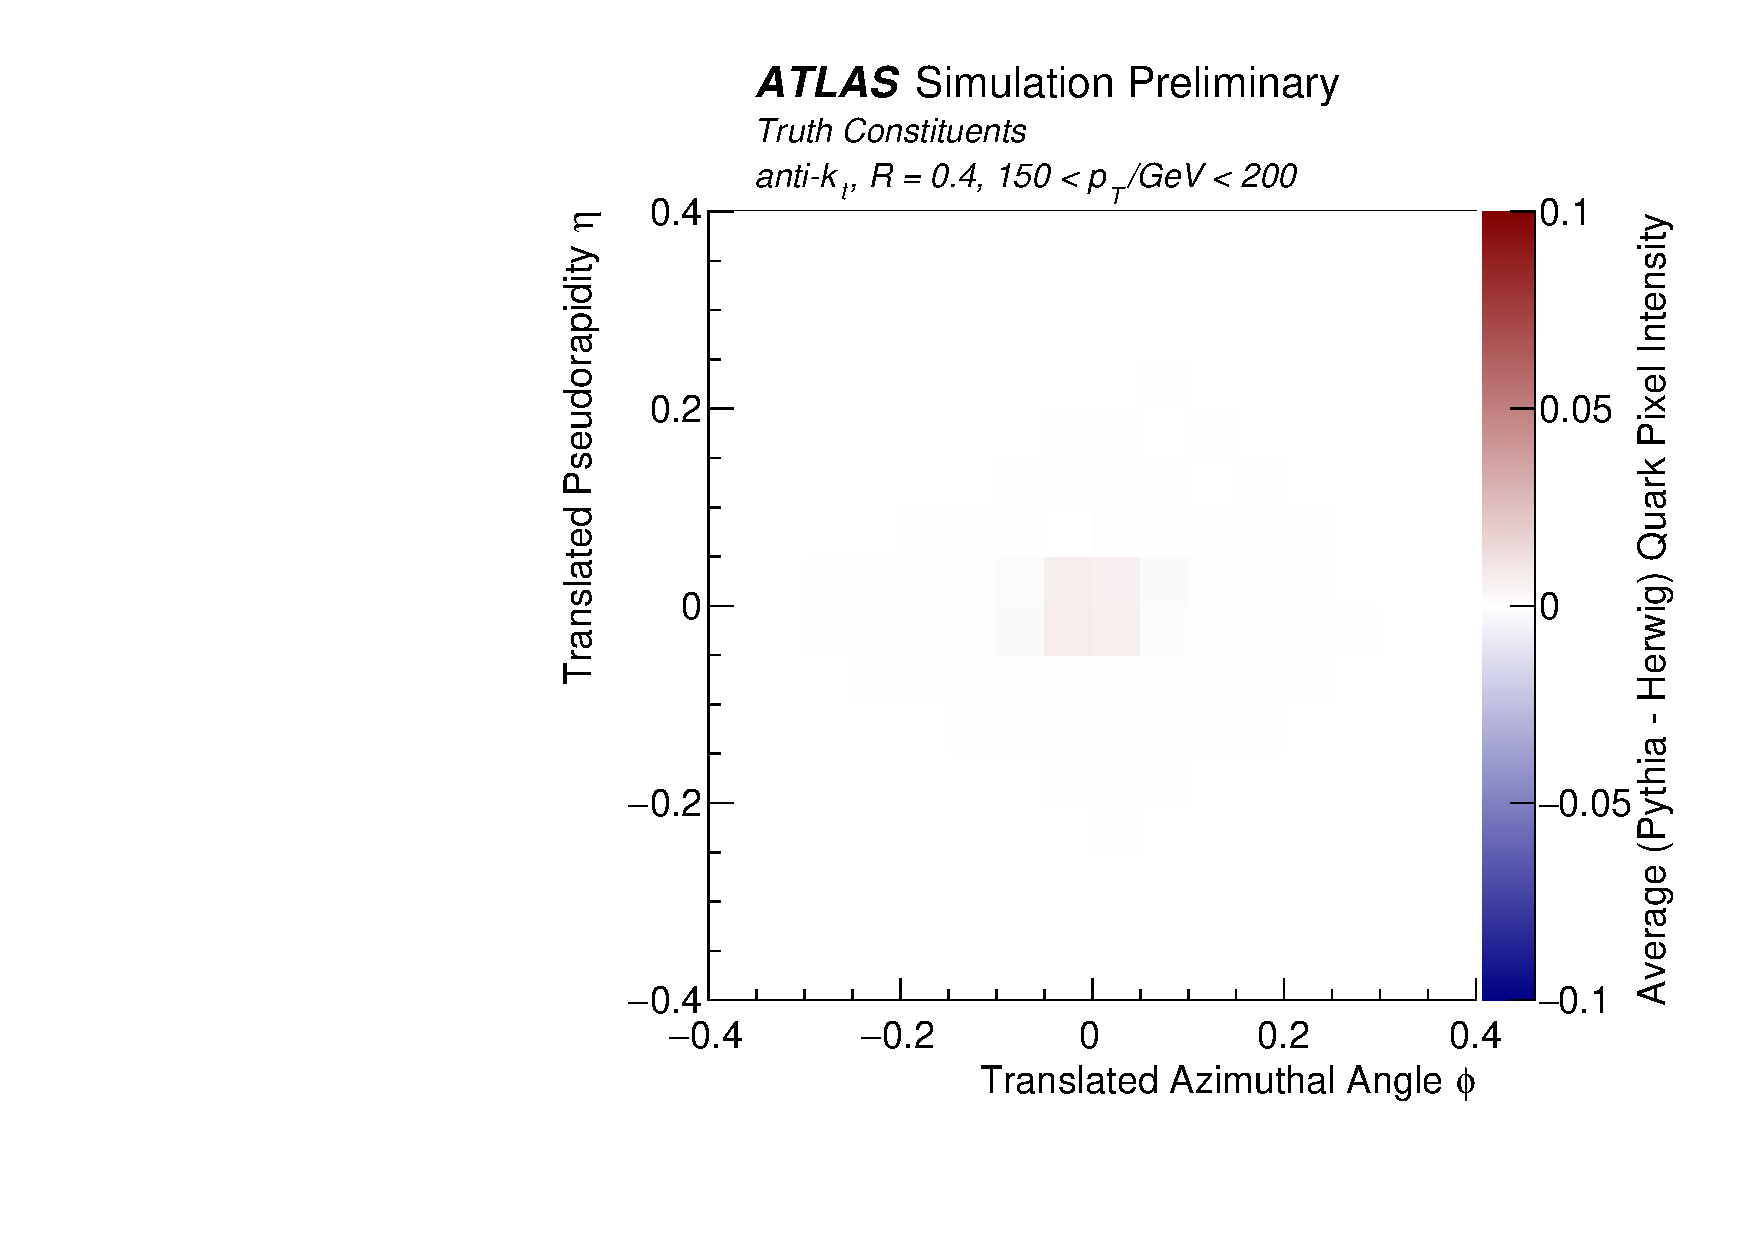
\includegraphics[width=0.33\textwidth]{figures/pythiasherpa/diff_truthq_pythiaherwig.pdf}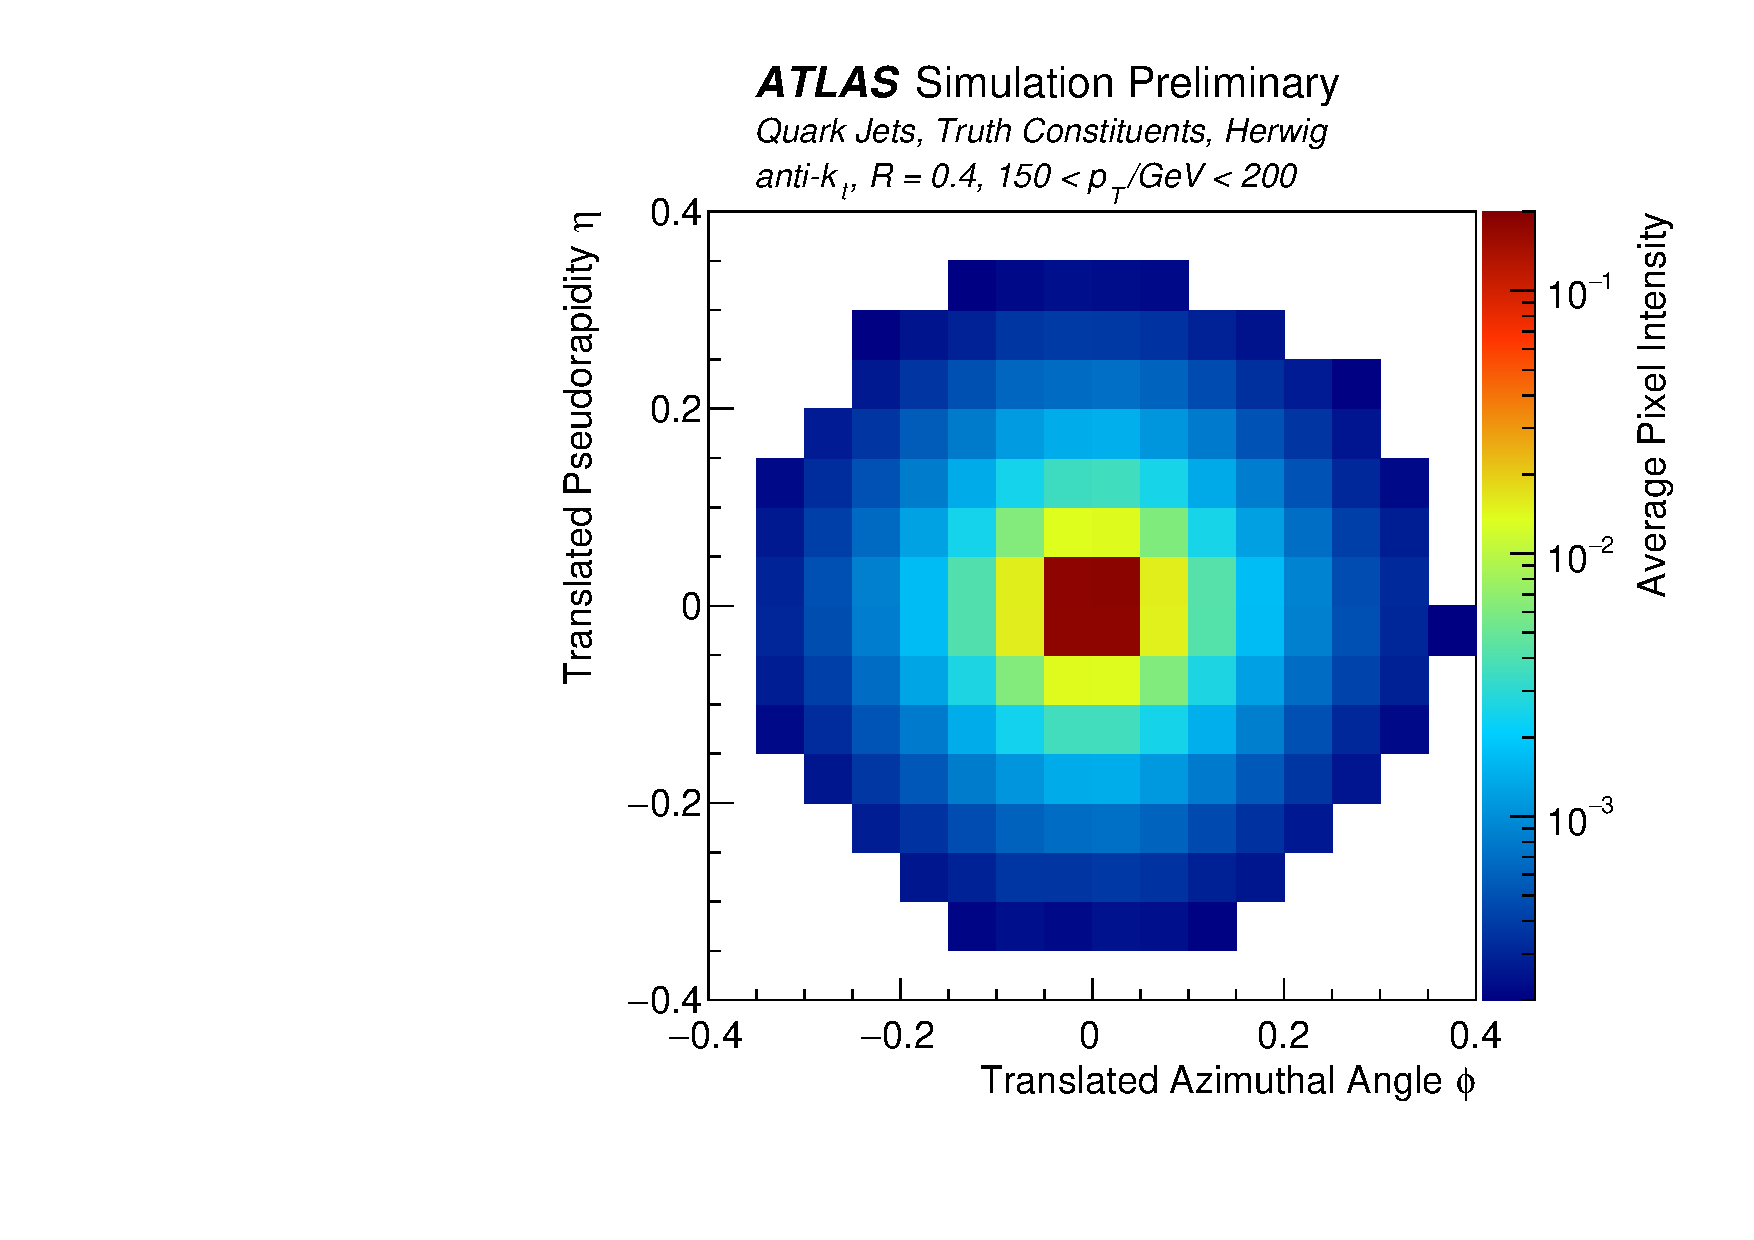
\includegraphics[width=0.33\textwidth]{figures/pythiasherpa/quark_truth_herwig.pdf}\\
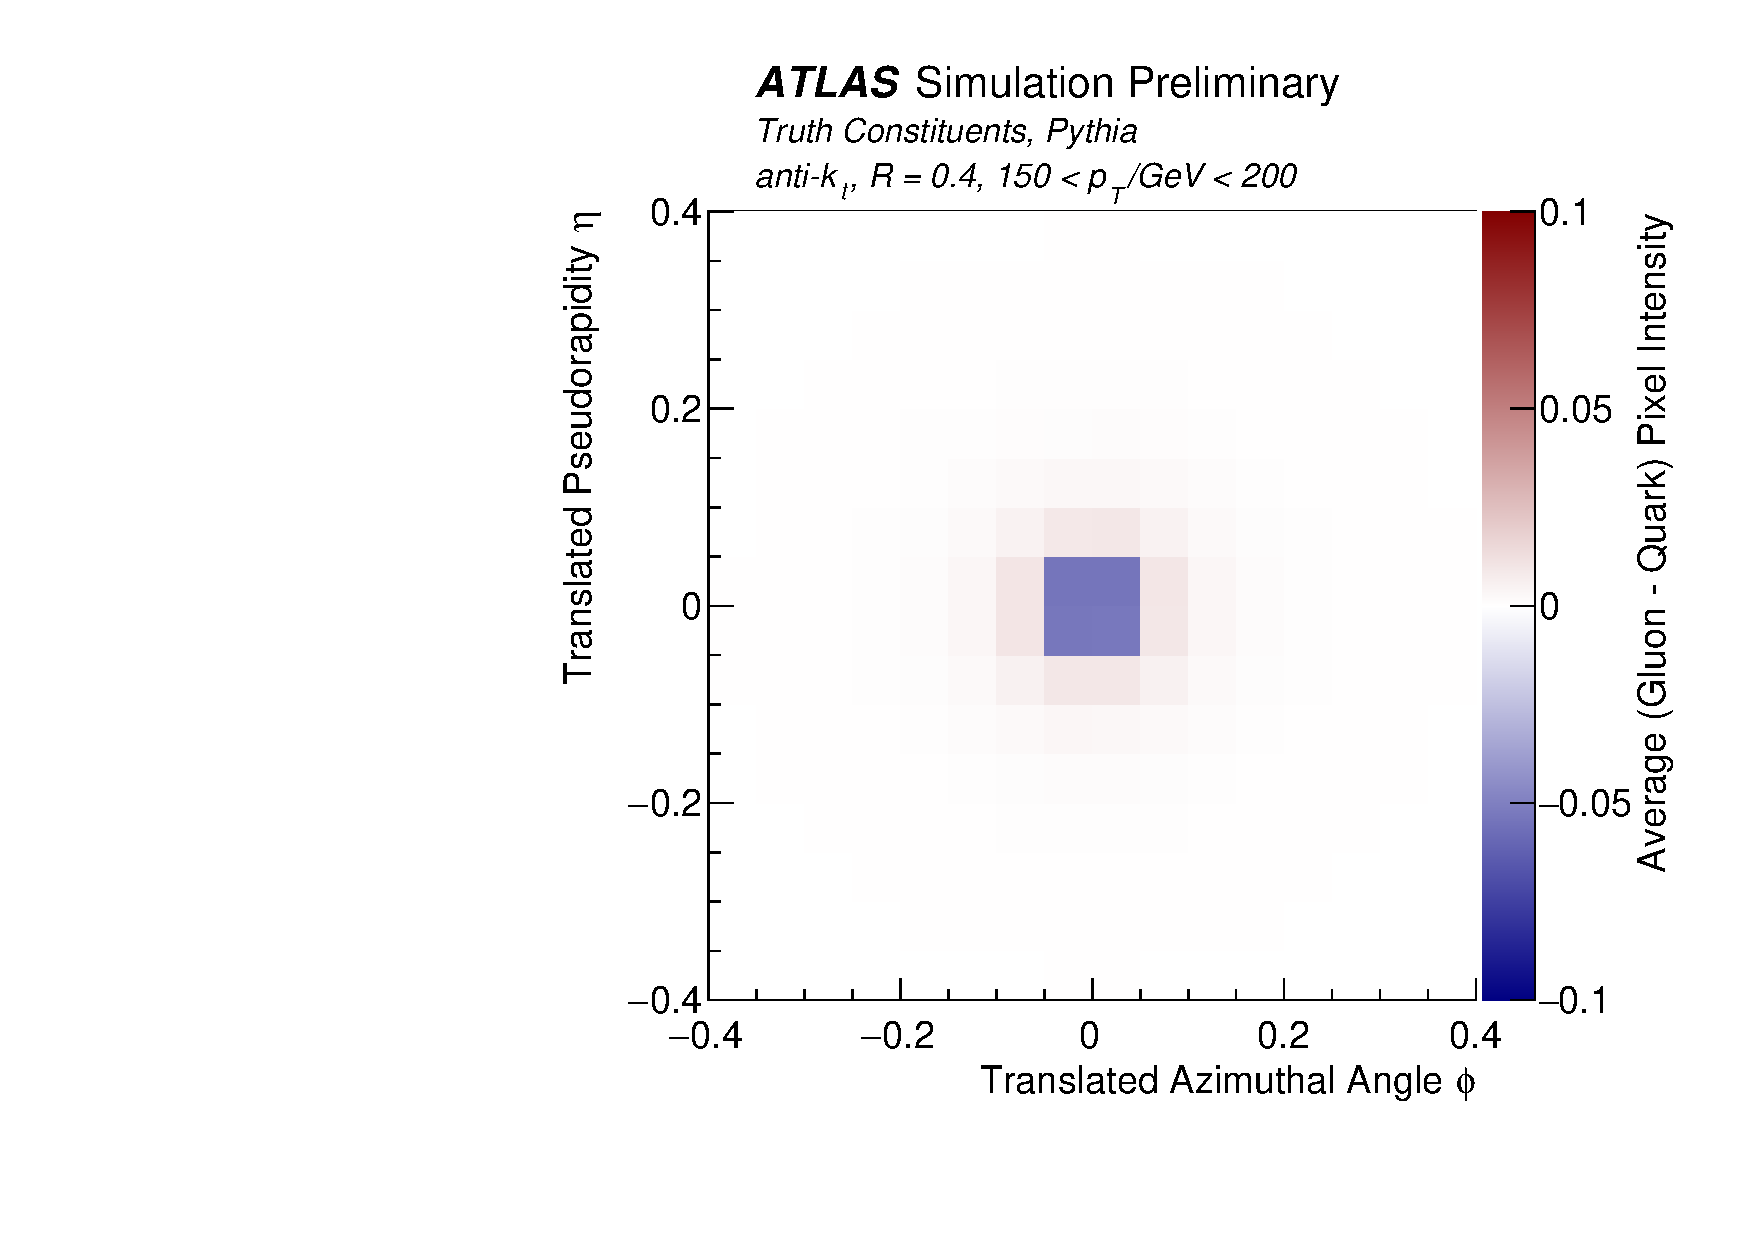
\includegraphics[width=0.33\textwidth]{figures/pythiasherpa/diff_truth_pythia.pdf}\hspace{54mm}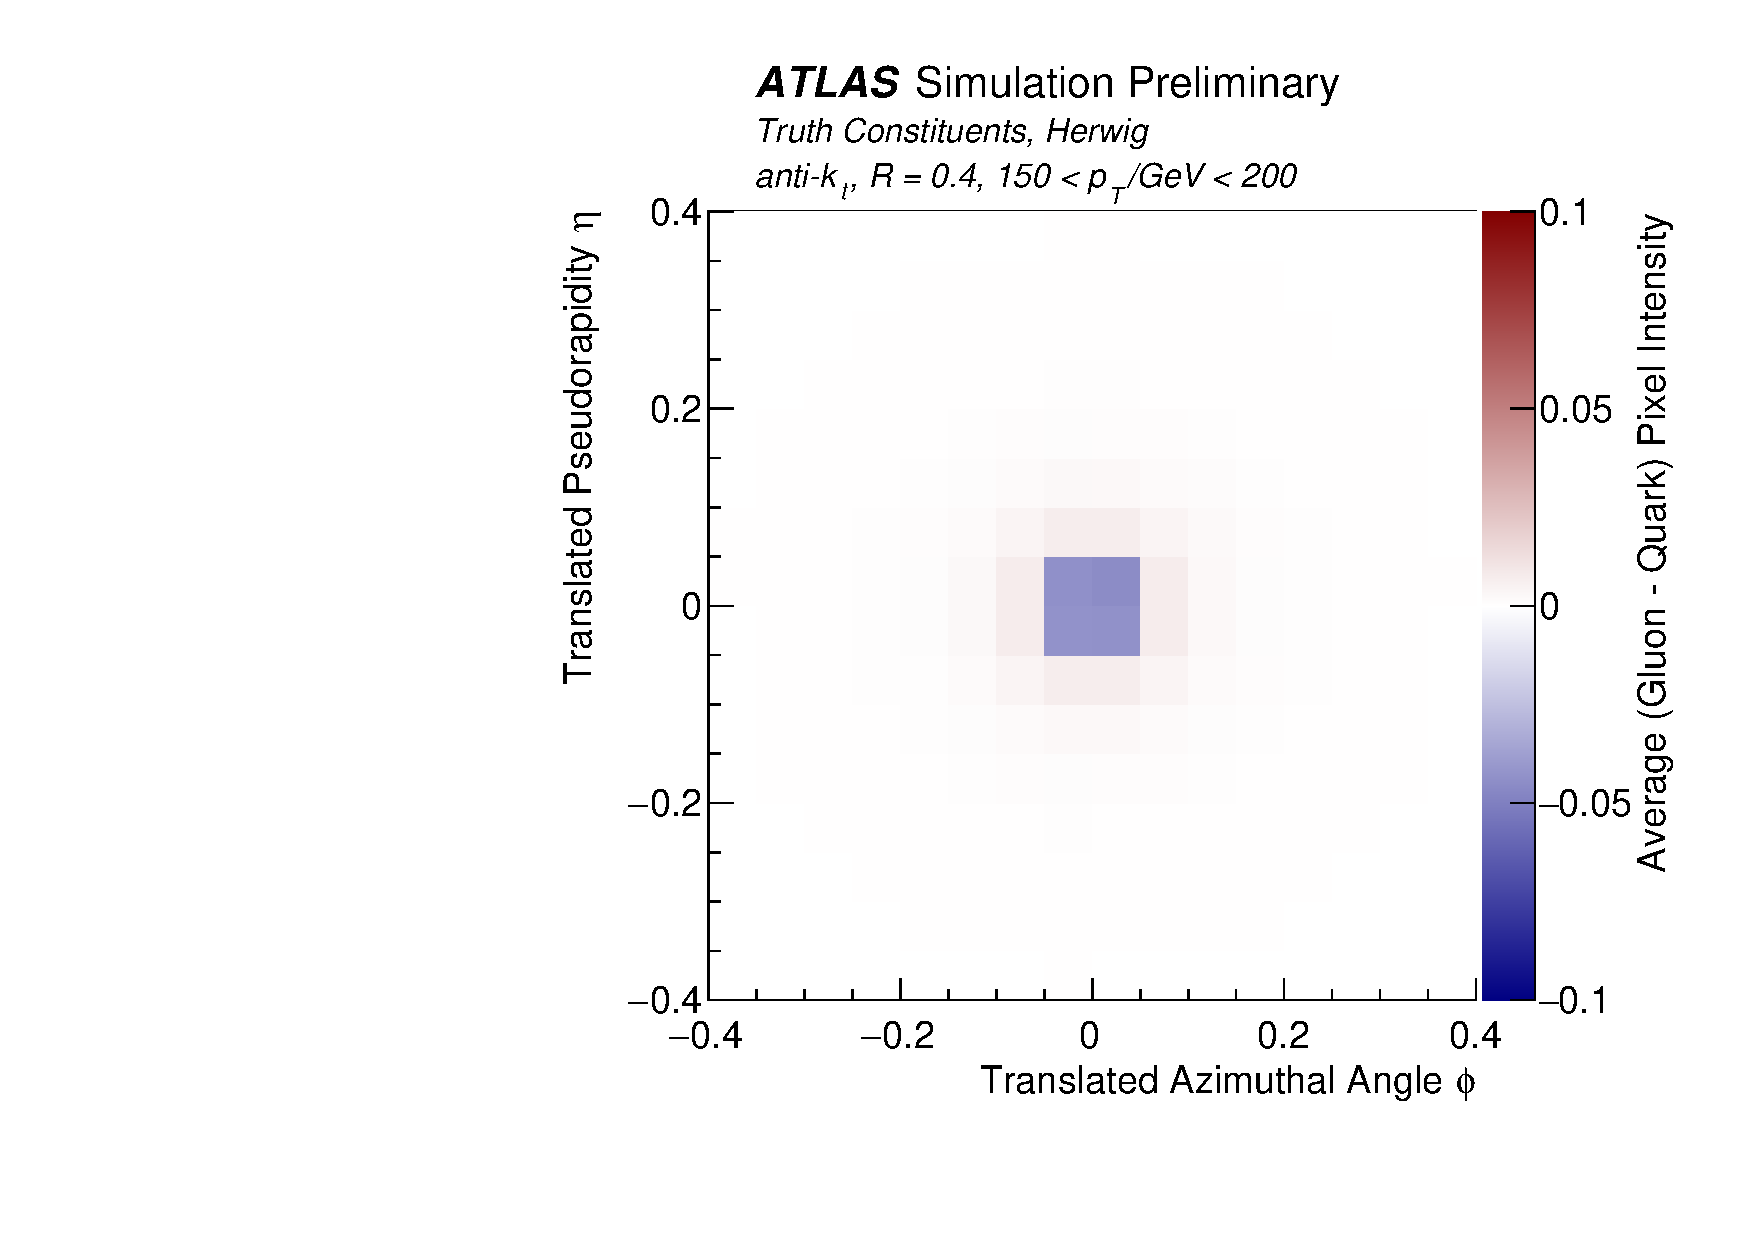
\includegraphics[width=0.33\textwidth]{figures/pythiasherpa/diff_truth_herwig.pdf}\\
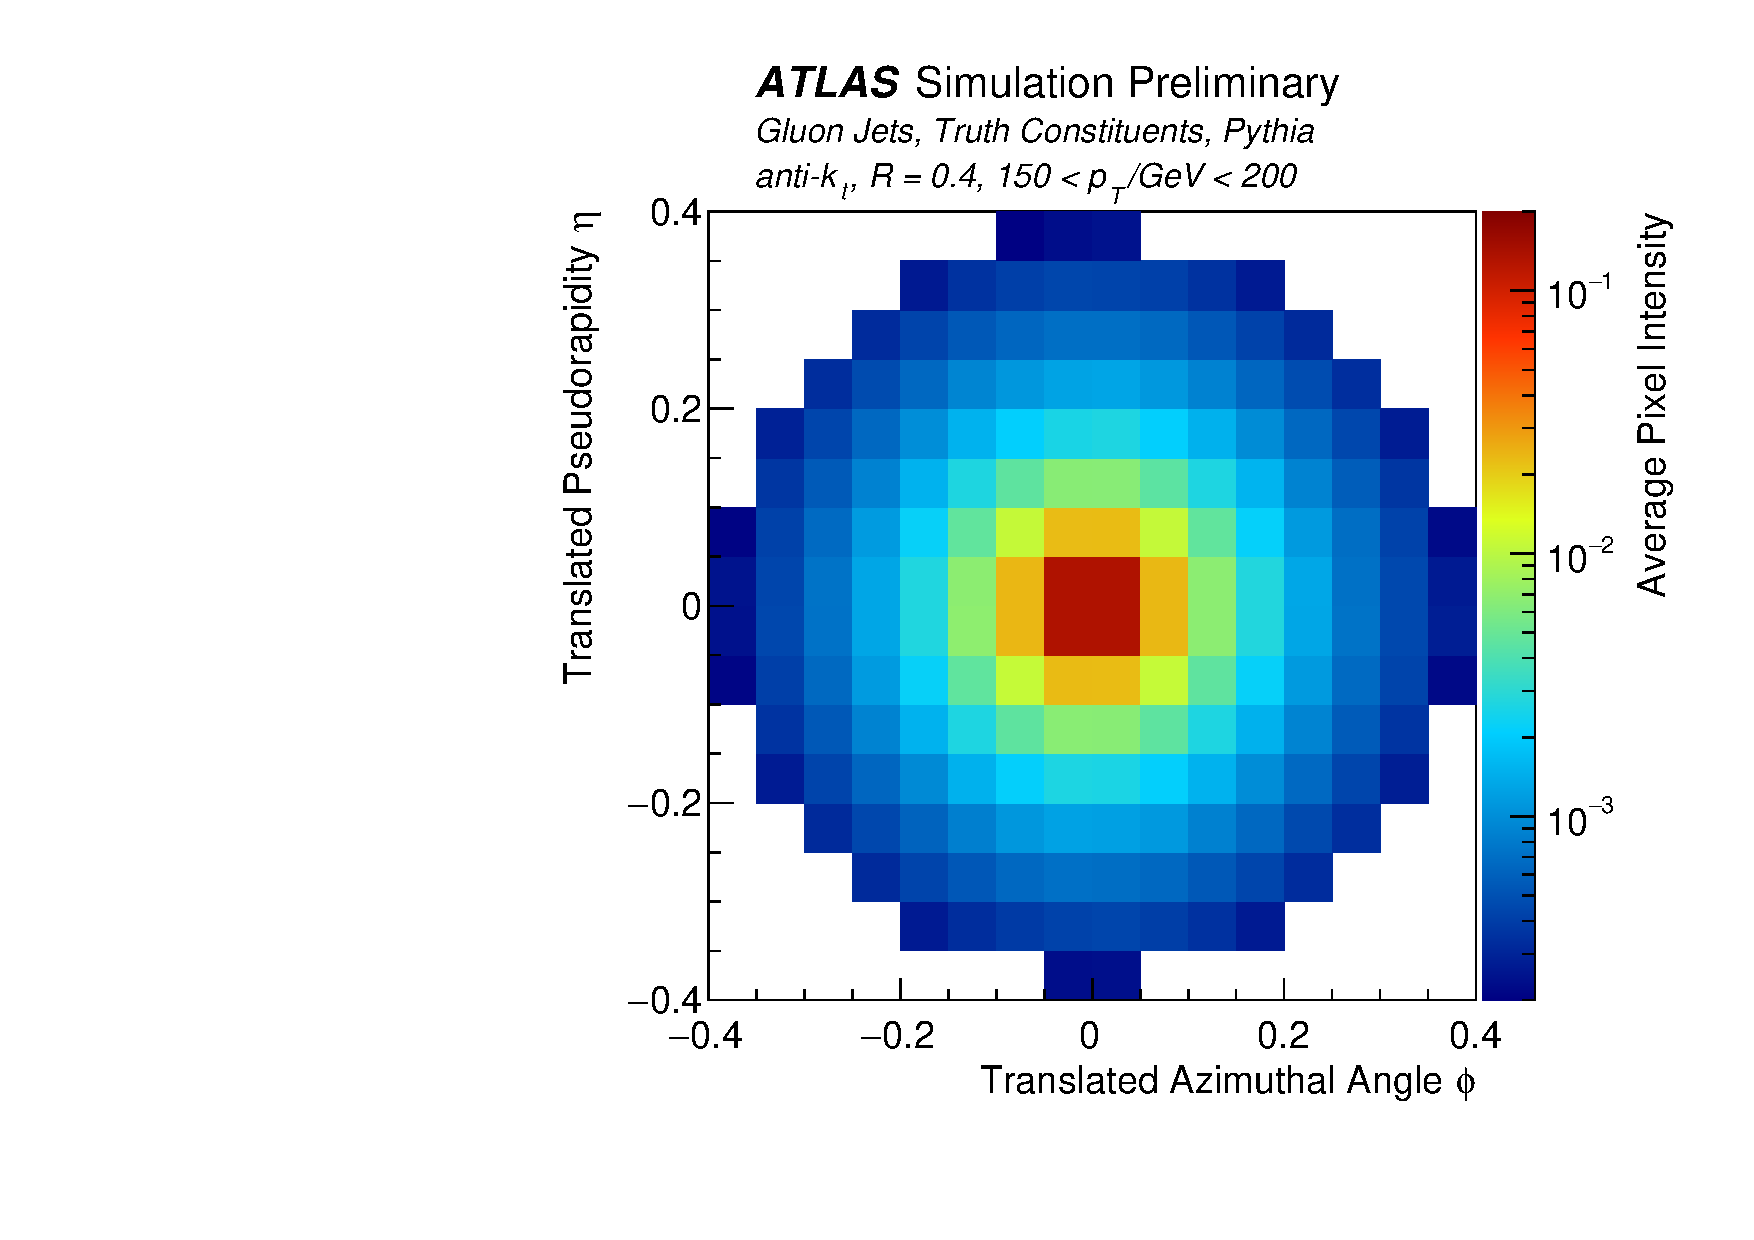
\includegraphics[width=0.33\textwidth]{figures/pythiasherpa/gluon_truth_pythia.pdf}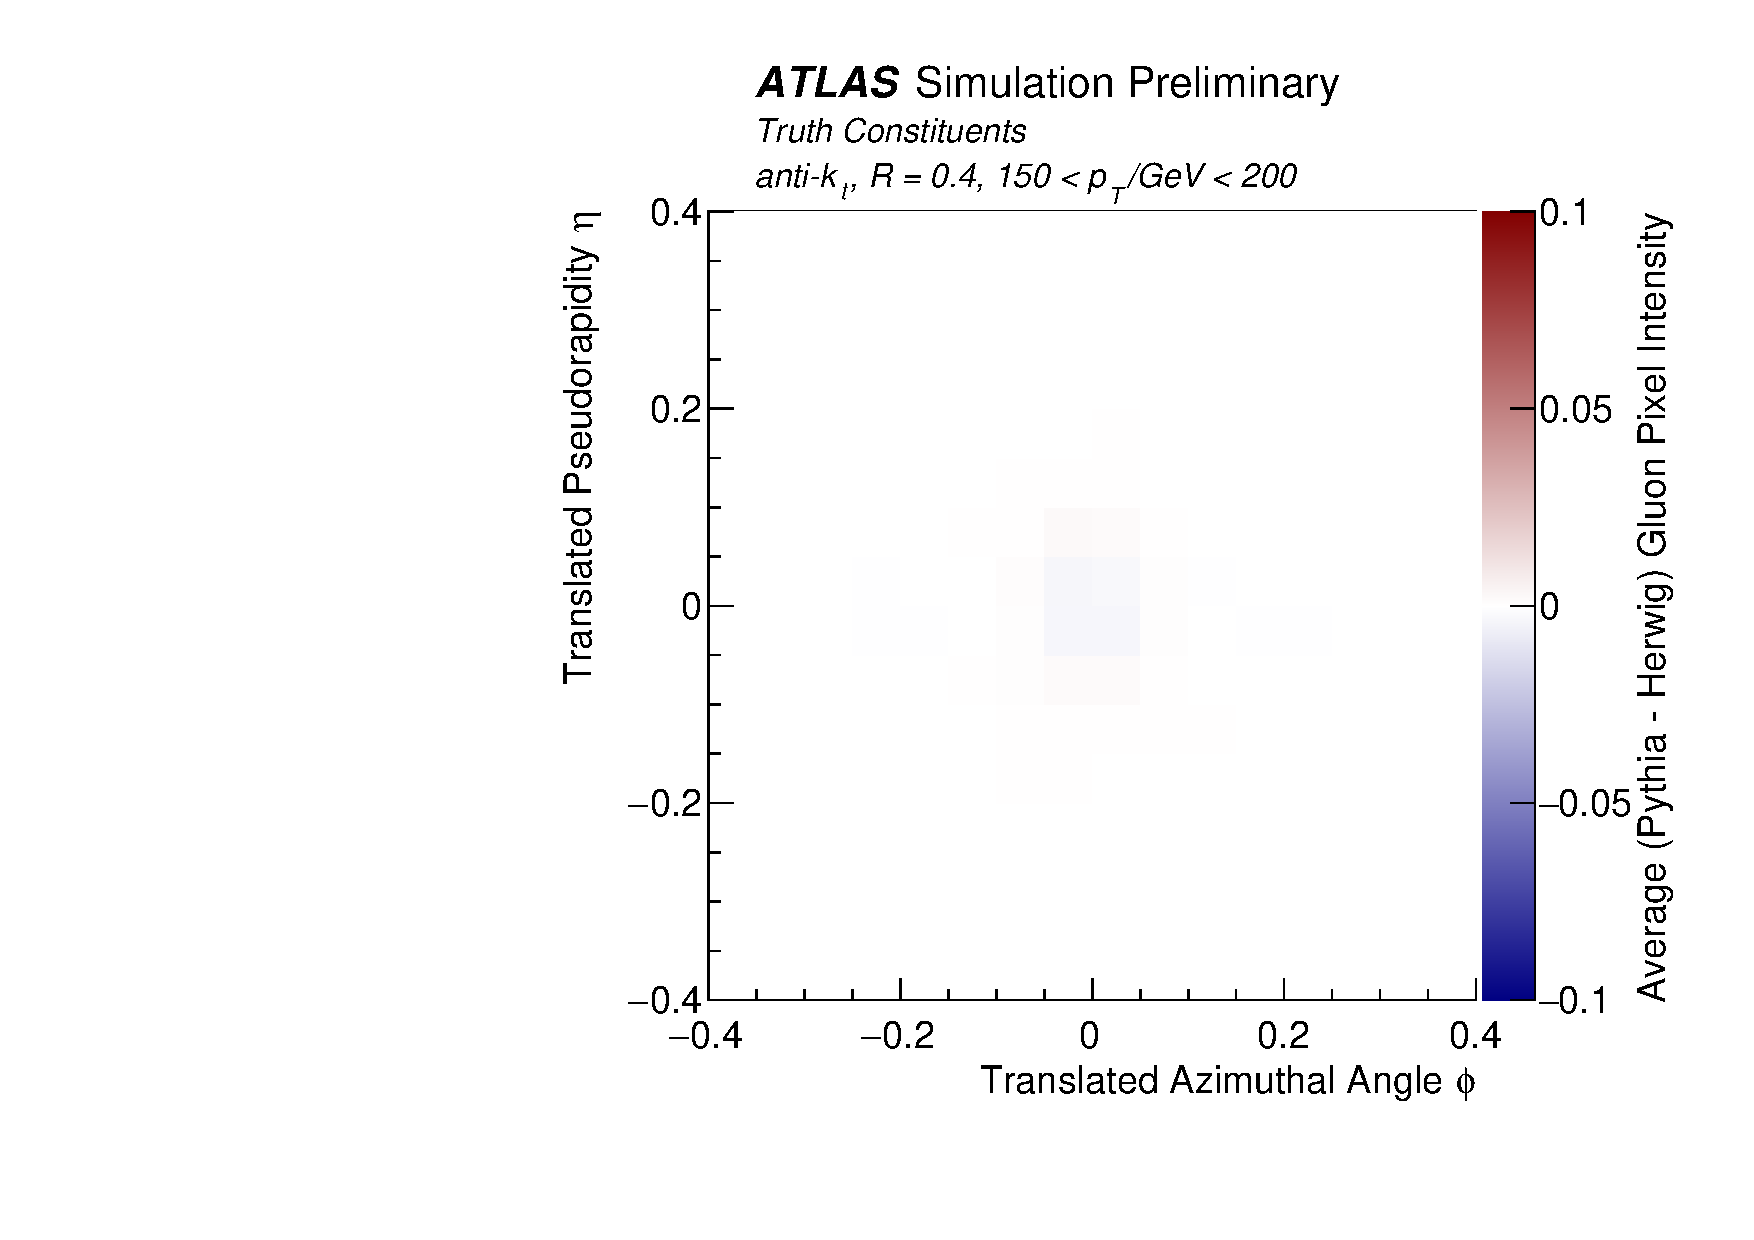
\includegraphics[width=0.33\textwidth]{figures/pythiasherpa/diff_truthg_pythiaherwig.pdf}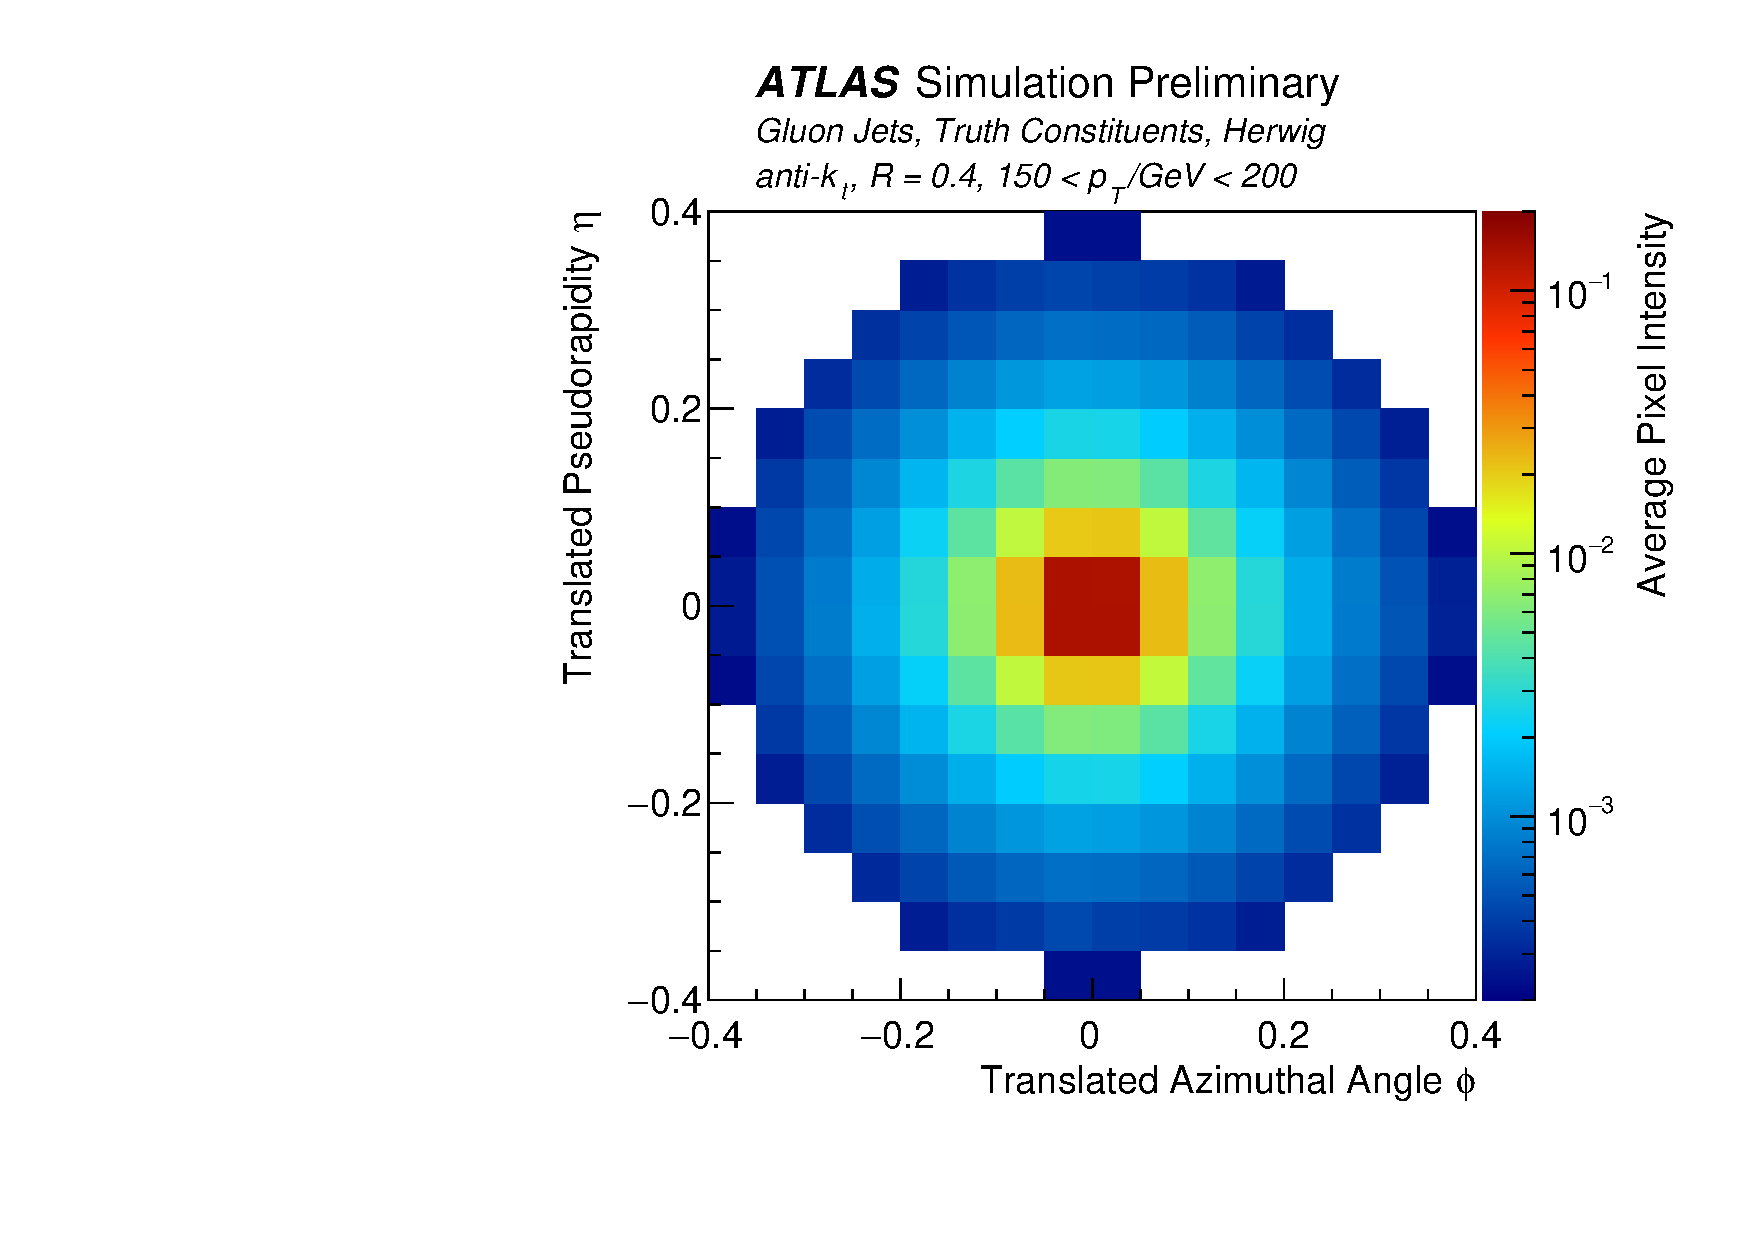
\includegraphics[width=0.33\textwidth]{figures/pythiasherpa/gluon_truth_herwig.pdf}
\caption{
The four corners show the average quark (top) and gluon (bottom) jet images, for jets generated with \textsc{Pythia} (left) and
and \textsc{Herwig} (right); the four plots on the edges show the difference between the adjacent plots,
for example the top plot shows the difference between the average quark jet in \textsc{Pythia} and
and \textsc{Herwig}.}
\label{fig:avg:pythiasherpa}
\end{center}
\end{figure}


\begin{figure}[h!]
\begin{center}
\subfloat[][]{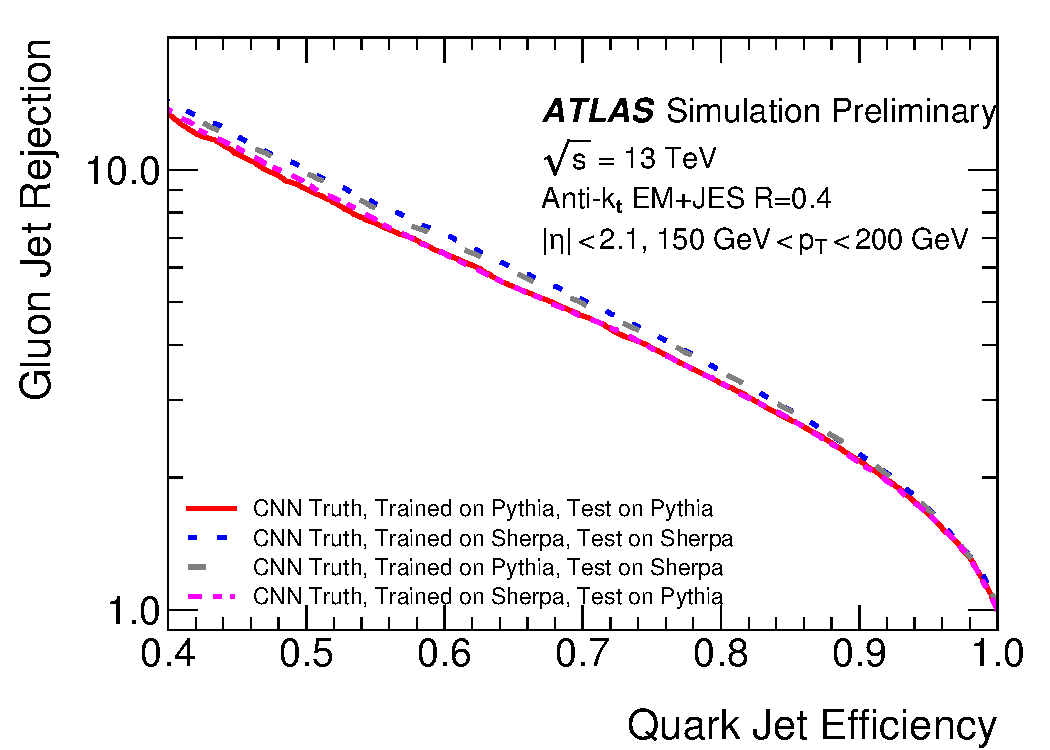
\includegraphics[width=0.5\textwidth]{figures/roc/ROC_pt150_200_gen_pythia_sherpa.pdf}\label{pythiasherpa}} 
\subfloat[][]{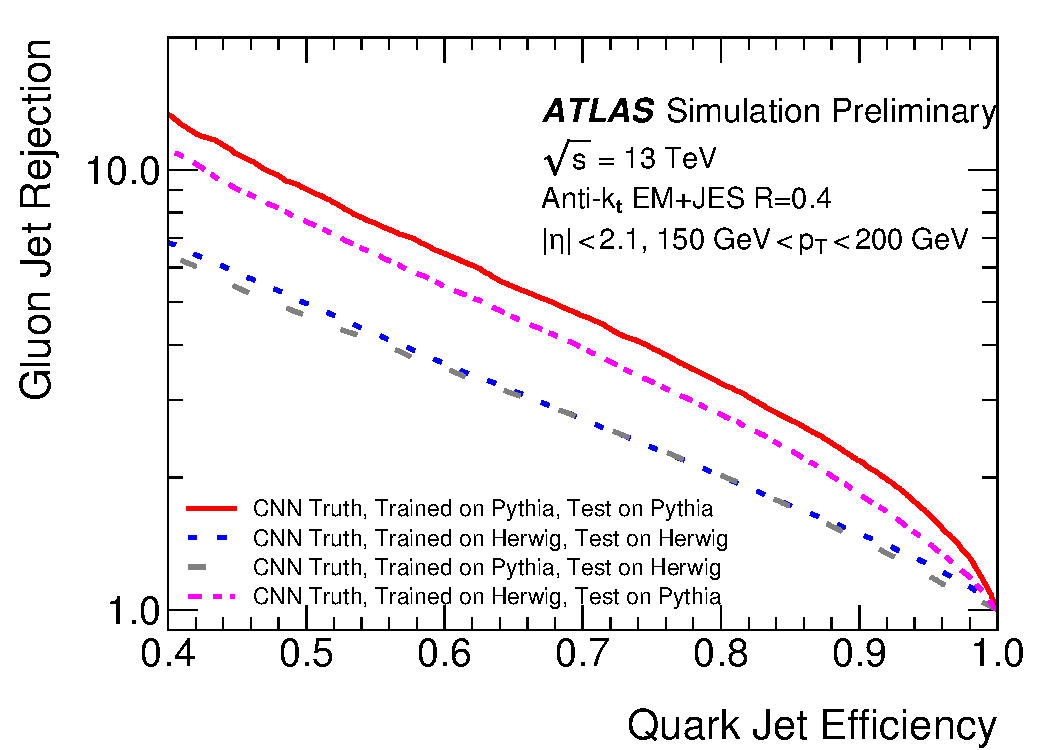
\includegraphics[width=0.5\textwidth]{figures/roc/ROC_pt150_200_gen_pythia_herwig.pdf}\label{pythiaherwig}} 
\caption{Gluon jet rejection as a function of the quark jet efficiency comparing \textsc{Pythia} to \protect\subref{pythiasherpa} \textsc{Sherpa}
and \protect\subref{pythiaherwig} \textsc{Herwig} for jets with $150<\pt<200~\GeV$.}
\label{fig:pythiasherpa}
\end{center}
\end{figure}


